\documentclass{article}
\usepackage[utf8]{inputenc}
\usepackage{amsmath}
\usepackage{amsfonts}
\usepackage{bbm}
\usepackage{graphicx}
\usepackage{subcaption}

\title{Computational Economics PS3}
\author{Yi Wu}
\date{January 2023}

\begin{document}
	
	\maketitle
	
	\section{Stationary Equilibrium}
	
	\subsection{Equilibrium Definition}
	
	The stationary equilibrium in Huggett (1996) is a set of $\{c_t, a_t, \mu_t, \phi, K, L, w, r, b, \tau\}$ s.t.
	\begin{itemize}
		\item Households maximize utility:
		\begin{gather*}
			\max \mathbb{E}\sum\limits_{t=1}^N \beta^t \frac{c_t^{1-\sigma}}{1-\sigma}\\
			s.t.\ c_t+a_{t+1}\le (1-\tau-\theta)e(z_t,t)w + [1+(1-\tau)r]a_t +b_t\\
			a_{t+1}\ge -\Bar{a}
		\end{gather*}
		where efficient labor $e(z_t, t)$ is defined as:
		\begin{equation*}
			e(z_t,t)=z_ty_t
		\end{equation*}
		and pension $b_t=\mathbbm{1}\{t\ge R\}b$.
		\item A representative firm maximizes its profit
		\begin{gather*}
			\max AK^\alpha N^{1-\alpha}-(r+\delta)K - wL
		\end{gather*}
		\item Population distribution follows the dynamic:
		\begin{gather*}
			\mu_{t+1} = \frac{\mu_t}{1+n}\\
			\sum\limits_{t=1}^N \mu_t = 1
		\end{gather*}
		\item Capital market clears:
		\begin{equation*}
			K=\frac{1}{1+n}\sum\limits_{t=1}^N \mu_t\int a_t'(a,z)d\phi_t(a,z)=\sum\limits_{t=1}^N \mu_t\int a\ d\phi_t(a,z)
		\end{equation*}
		\item Labor market clears:
		\begin{equation*}
			L = \sum\limits_{t=1}^N \mu_t\int e(z,t)d\phi_t(a,z)
		\end{equation*}
		\item Pension system clears:
		\begin{equation*}
			\theta wL=b\sum\limits_{t=R}^N\mu_t
		\end{equation*}
		\item Government budget holds:
		\begin{equation}
			G=\frac{G}{Y}Y=\tau(Y-\delta K)
		\end{equation}
	\end{itemize}
	
	The parameters in the model is in Table \ref{tab:params}.
	
	\begin{table}[h]
		\centering
		\begin{tabular}{c|c}
			Parameter & Value \\
			$\alpha$ & 0.36\\
			$\beta$ & 0.994\\
			$\sigma$ & 1.5\\
			$\delta$ & 0.06\\
			$A$ & 0.6\\
			$n$ & 0.012/0.001\\
			$N$ & 79\\
			$R$ & 54\\
			$\Bar{a}$ & 0\\
			$\theta$ & 0.1\\
			$\frac{G}{Y}$ & 0.195\\
		\end{tabular}
		\caption{Parameters}
		\label{tab:params}
	\end{table}
	
	\subsection{Numerical Stationary Equilibrium}
	The numerical algorithm is similar to Huggett (1996) excepted that I use on-the-grid policy and non-linear asset grids:
	\begin{equation}
		\log (a[i+1]+\Tilde{a}) - \log(a[i]+\Tilde{a}) = \frac{1}{anum-1}\left\{\log (amax+\Tilde{a}) - \log(-\Bar{a}+\Tilde{a})\right\}
	\end{equation}
	where $\Tilde{a}=0.5$, $amax=200$, $anum=2000$.
	The non-linearity leads to more grids when $a$ is small, so the precision of policy function is more accurate for financially constrained agents.
	
	The numeric value of aggregate variables when $n=0.012$ is in Table \ref{tab:se}.
	
	\begin{table}[h]
		\centering
		\begin{tabular}{c|c}
			Variable & Value \\
			$K$ & 3.730\\
			$L$ & 0.529\\
			$Y$ & 0.641\\
			$b$ & 0.177\\
			$w$ & 0.776\\
			$r$ & 0.00188\\
			$\tau$ & 0.300\\
		\end{tabular}
		\caption{Stationary Equilibrium}
		\label{tab:se}
	\end{table}
	
	The decision rule of cohorts with age 1, $R$, $N/3$ when $z$ is lowest, median, highest are in Figure \ref{fig:rule}.
	The policy function is kinky because I didn't interpolate the value function and let the policy function be off the grid as described in Huggett (1996).
	It can be seen from the graph that those who has little asset, low efficient labor, or those who are young or old are more likely be limited by no borrowing constraint.
	Those agents who have large labor income can save even if they don't have any asset before.
	
	\begin{figure}[h]
		\centering
		\begin{subfigure}{0.32\textwidth}
			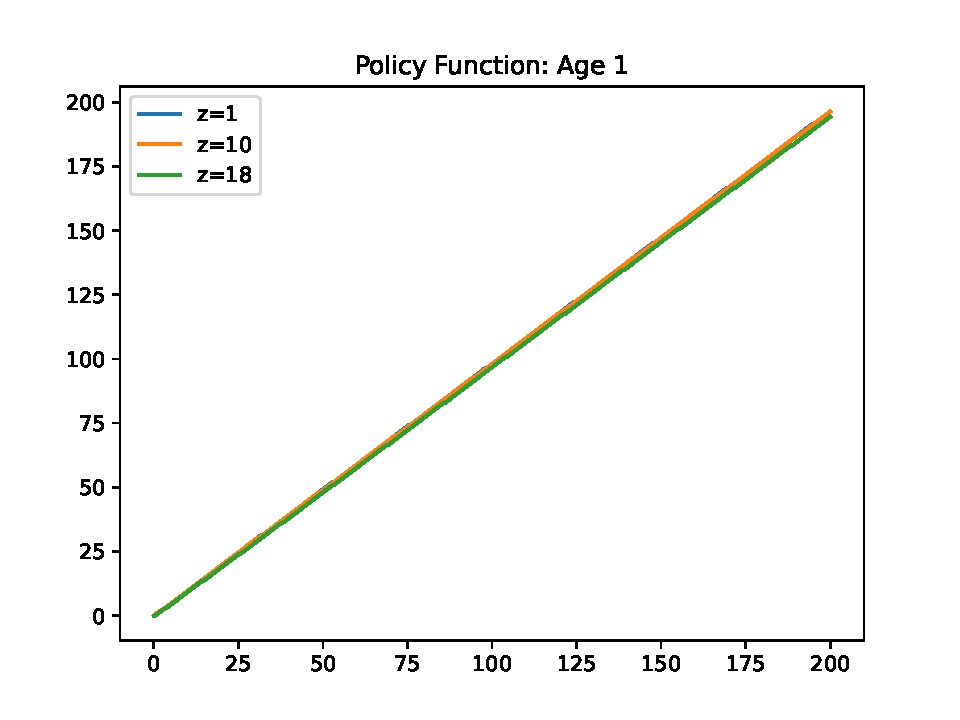
\includegraphics[width=0.95\textwidth]{../figures/policy_1.pdf}
		\end{subfigure}
		\begin{subfigure}{0.32\textwidth}
			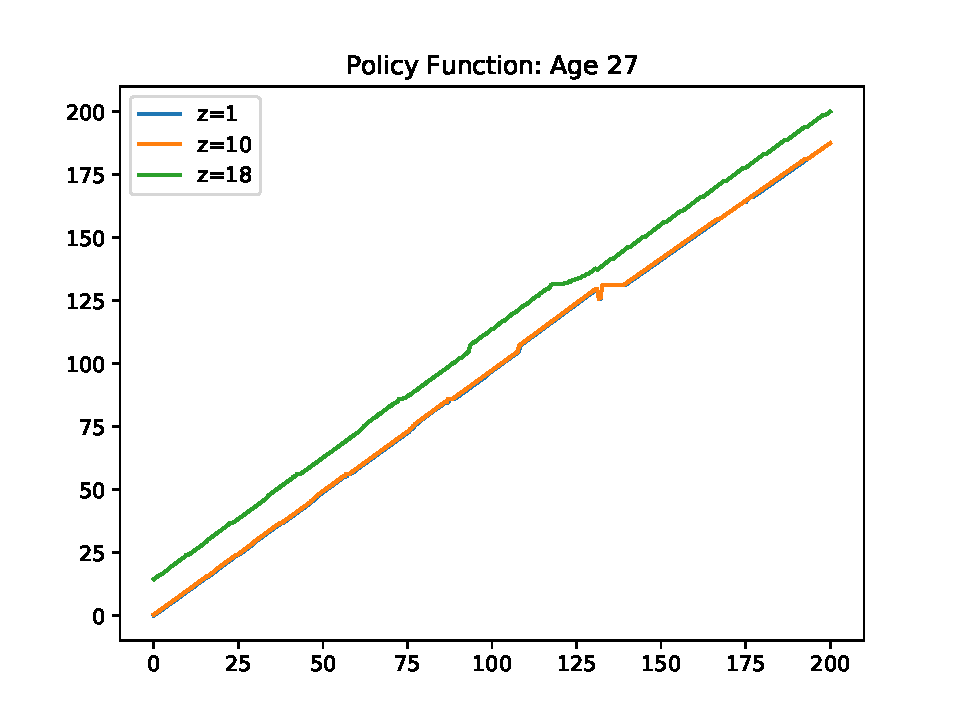
\includegraphics[width=0.95\textwidth]{../figures/policy_27.pdf}
		\end{subfigure}
		\begin{subfigure}{0.32\textwidth}
			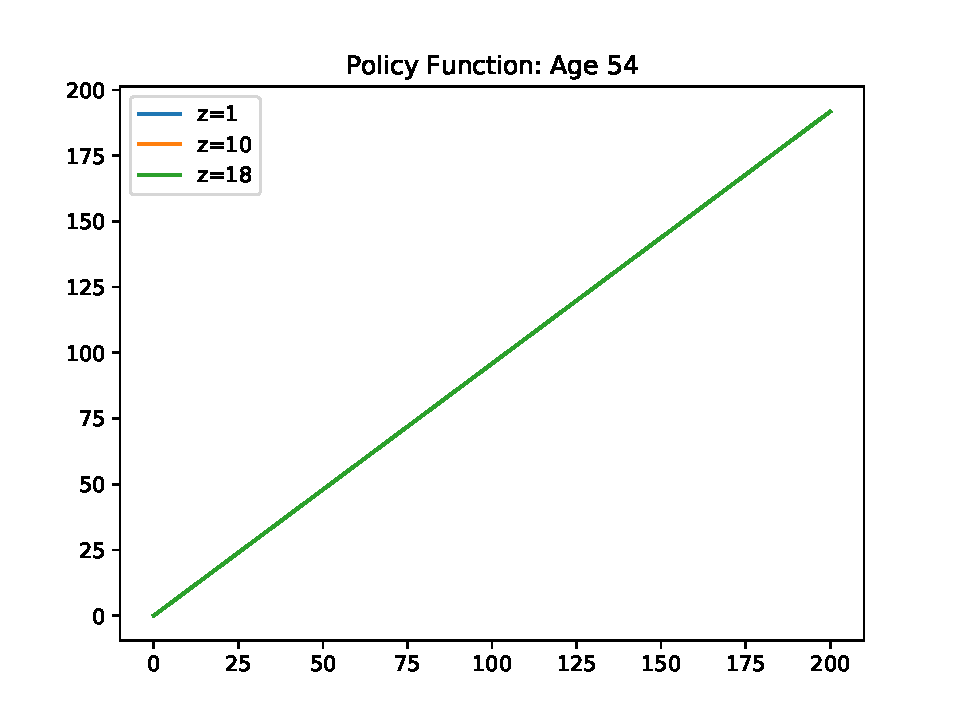
\includegraphics[width=0.95\textwidth]{../figures/policy_54.pdf}
		\end{subfigure}
		\caption{Policy Function}
		\label{fig:rule}
	\end{figure}
	
	The Lorenz curve is in Figure \ref{fig:lorenz}.
	And other distribution-related statistics are in Table \ref{tab:gini}.
	Compared with Table 1 in Huggett (1996), we can see that the model underestimates the wealth inequality.
	From Table \ref{tab:gini}, the bias most comes from the top 1\%.
	
	\begin{figure}[h]
		\centering
		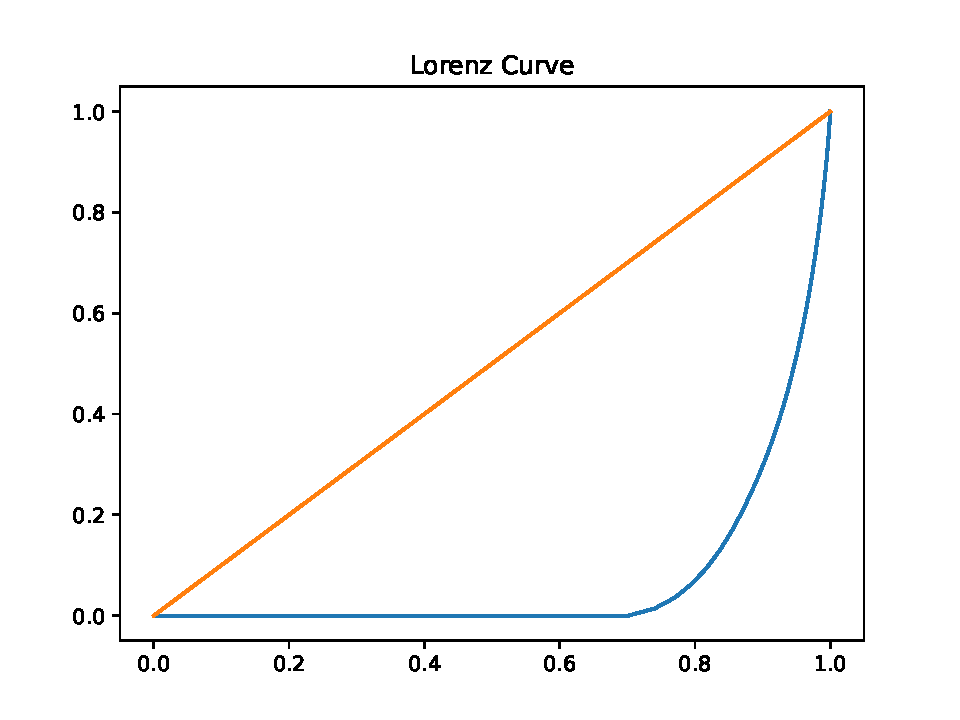
\includegraphics[width=0.9\textwidth]{../figures/Lorenz.pdf}
		\caption{Lorenz Curve}
		\label{fig:lorenz}
	\end{figure}
	
	\begin{table}[h]
		\centering
		\begin{tabular}{c|c|c|c|c|c|c|c}
			Percentage Wealth in Top & 1\% & 5\% & 20\% & 40\% & 60\% & 80\% & Wealth Gini\\
			U.S. (Huggett, 1996) & 28\% & 49\% & 75\% & 89\% & 96\% & 99\% & 0.72\\
			model & 7.8\% & 25.2\% & 59.3\% & 82.3\% & 94.1\% & 99.1\% & 0.577
		\end{tabular}
		\caption{Caption}
		\label{tab:gini}
	\end{table}
	
	The mean and variance of log labor income, total income, and consumption conditional on age are in Figure \ref{fig:mom}.
	Life cycle hypothesis suggests that agents will save in the middle age and borrow at young and old age.
	This corresponds to the movement of the mean of the wealth.
	The variance of labor income is exogenous, and it explains a large part of total income variance before the retirement.
	A short period before the retirement, because the labor share of the income declines, the variance of total income surges.
	After the retirement, equal pension smooths the variance of income.
	
	The mean of consumption raises before mid-age, and then remain stable.
	This curve reflects the permanent income hypothesis: agents will smooth their consumption if they are not financially constrained.
	Before mid-age, they are financially constrained, so there is an increasing curve.
	After they accumulates some assets, they can handle the income shock by consuming some of the assets.
	The variance of consumption reaches its peak before the the peak of total income because those who earn more before retirement need also to save more to smooth their consumption path.
	\begin{figure}[h]
		\centering
		\begin{subfigure}{0.48\textwidth}
			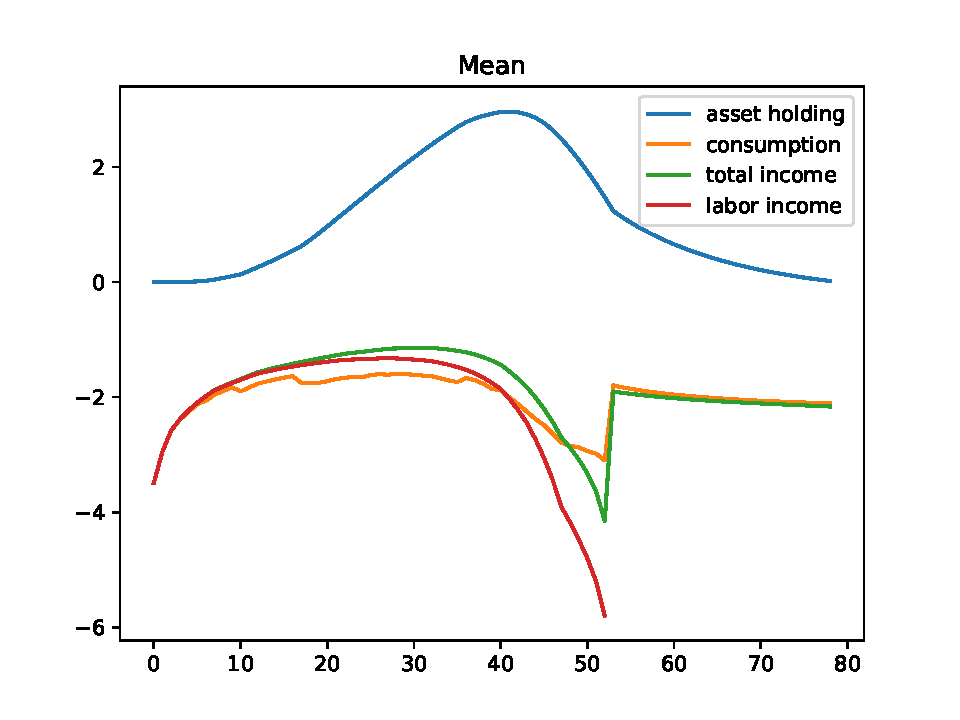
\includegraphics[width=0.95\textwidth]{../figures/mean.pdf}
		\end{subfigure}
		\begin{subfigure}{0.48\textwidth}
			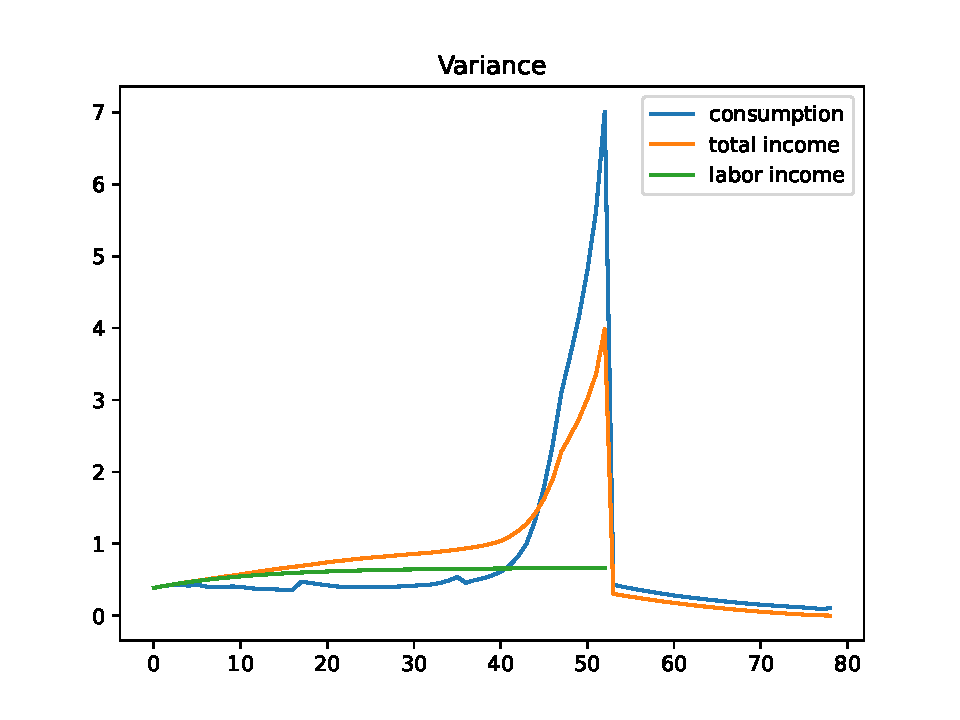
\includegraphics[width=0.95\textwidth]{../figures/variance.pdf}
		\end{subfigure}
		\caption{Moments of Variables}
		\label{fig:mom}
	\end{figure}
	\section{Comparative Statics Analysis}
	
	The aggregate variables in stationary equilibrium given different $n$ are in Table \ref{tab:se2}.
	When population growth rate $n$ goes down, the aggregate labor supply declines.
	On the other side, the elderly are tend to be savers, so aggregate capital increases.
	Overall, the labor supply effect dominates the saving effect: the output declines when population growth slows down.
	Since the output declines, there is mainly a welfare loss of moving the equilibrium.
	
	The welfare differences are plotted in Figure \ref{fig:lamda}.
	It's defined as:
	\begin{equation}
		\lambda(a,z,t)=\left[ \frac{V(a,z,t|n=0.001)}{V(a,z,t|n=0.012)} \right]^{\frac{1}{1-\sigma}}- 1
	\end{equation}
	we can see for the young cohorts, the welfare effect is minor compared with older cohorts since most of them have little assets.
	The largest intra-cohort welfare heterogeneity comes from the working-age cohorts.
	This is because the efficiency heterogeneity has the largest impact on their wealth at that time.
	Those with higher efficiency are less affected by the slow-down of the population growth, because the rising wage increases their wealth.
	For the retired, the welfare loss is large because their pension shrinks.
	Those with little assets suffer more from the pension shrink because they don't have income from elsewhere.
	\begin{figure}[h]
		\centering
		\begin{subfigure}{0.32\textwidth}
			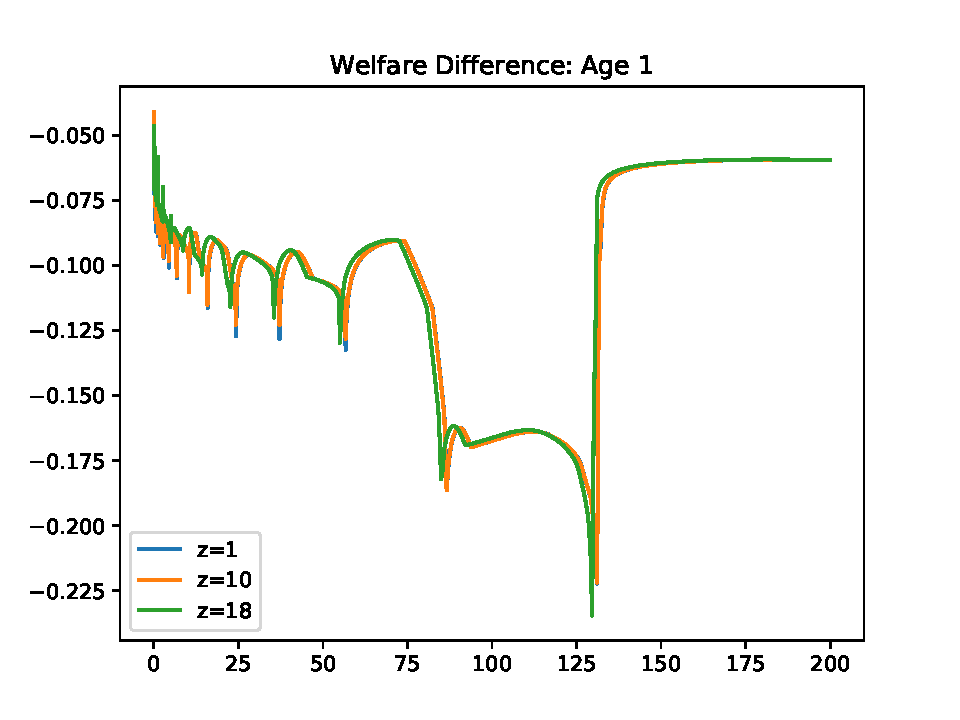
\includegraphics[width=0.95\textwidth]{../figures/lamda_1.pdf}
		\end{subfigure}
		\begin{subfigure}{0.32\textwidth}
			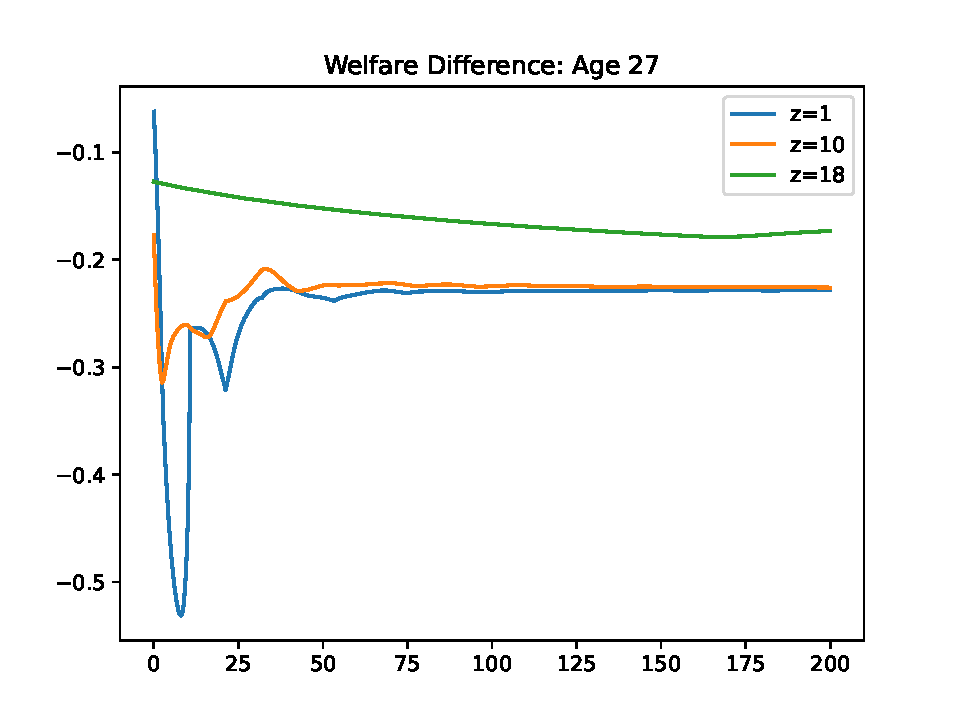
\includegraphics[width=0.95\textwidth]{../figures/lamda_27.pdf}
		\end{subfigure}
		\begin{subfigure}{0.32\textwidth}
			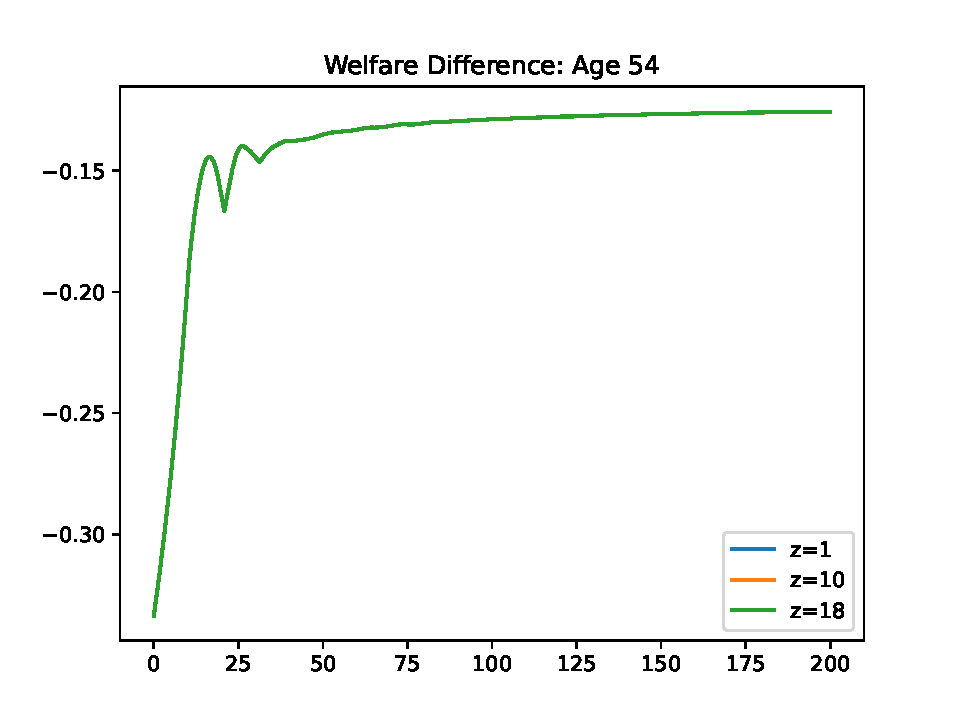
\includegraphics[width=0.95\textwidth]{../figures/lamda_54.pdf}
		\end{subfigure}
		\caption{Welfare Difference}
		\label{fig:lamda}
	\end{figure}
	
	\begin{table}[h]
		\centering
		\begin{tabular}{c|c|c}
			Variable & $n=0.012$ & $n=0.001$ \\
			$K$ & 3.730 & 3.882\\
			$L$ & 0.529 & 0.461\\
			$Y$ & 0.641 & 0.596\\
			$b$ & 0.177 & 0.119\\
			$w$ & 0.776 & 0.827\\
			$r$ & 0.00188 & -0.00475\\
			$\tau$ & 0.300 & 0.320\\
		\end{tabular}
		\caption{Stationary Equilibrium Given Different $n$}
		\label{tab:se2}
	\end{table}
	
	Table \ref{tab:gini2} compares the inequality regard to different $n$.
	
	\begin{table}[h]
		\centering
		\begin{tabular}{c|c|c|c|c|c|c|c}
			Percentage Wealth in Top & 1\% & 5\% & 20\% & 40\% & 60\% & 80\% & Wealth Gini\\
			U.S. (Huggett, 1996) & 28\% & 49\% & 75\% & 89\% & 96\% & 99\% & 0.72\\
			$n=0.012$ & 7.8\% & 25.2\% & 59.3\% & 82.3\% & 94.1\% & 99.1\% & 0.577\\
			$n=0.001$ & 7.5\% & 24.3\% & 57.8\% & 81.1\% & 93.4\% & 98.9\% & 0.562
		\end{tabular}
		\caption{Inequality at Different $n$}
		\label{tab:gini2}
	\end{table}
	The inequality in the second case is smaller.
	Maybe it's because the return of assets in lower in the second case, which gives the gifted less advantage to their accumulate their fortune.
\end{document}
